\documentclass[11pt,a4paper]{article}
\usepackage[T1]{fontenc}
\usepackage[utf8]{inputenc}
\renewcommand{\rmdefault}{ptm}
\usepackage{graphicx}
\usepackage[a4paper,left=21mm,right=21mm,top=21mm,bottom=21mm,footskip=10mm]{geometry}
\setlength{\parindent}{0pt}
\setlength{\parskip}{5pt}
\emergencystretch=2em
\setlength{\fboxrule}{0.6pt}
\pagestyle{plain}
\makeatletter
\newcommand{\LenToUnit}[1]{\strip@pt\dimexpr#1\relax}
\makeatother
% Draw the same border on every shipped page, including the cover.
\AddToHook{shipout/background}{%
  \setlength{\unitlength}{1pt}%
  \put(25,-\LenToUnit{\dimexpr\paperheight-25pt\relax}){%
    \framebox(\LenToUnit{\dimexpr\paperwidth-50pt\relax},\LenToUnit{\dimexpr\paperheight-50pt\relax}){}}}
\newcommand{\reportheading}[1]{\par\vspace{4pt}{\large\bfseries #1}\par\vspace{1pt}}
\newcommand{\reportsubheading}[1]{\par\vspace{2pt}{\normalsize\bfseries #1}\par}
\begin{document}
\begingroup
\fontsize{15}{18}\selectfont
\begin{center}
\vspace*{5mm}
{\fontsize{19}{23}\selectfont\bfseries QubitChat: Intelligent Document Question Answering with Grover-Inspired Evidence Selection\par}
\vfill
UROP Project submitted to the\\
{\bfseries SRM University -- AP, Andhra Pradesh}\\[2mm]
for the partial fulfillment of the requirements to award the degree of\\[1mm]
{\bfseries Bachelor of Technology in\\ Computer Science and Engineering}\\[2mm]
School of Engineering and Sciences\par
\vfill
{\bfseries Submitted by}\\[1mm]
Bala Rakesh Gundapaneni \textbar{} AP23110010003\\
Jagadeeshbabu Borru \textbar{} AP23110010058\\
Abdul Basith Syed \textbar{} AP23110011061\\
\vfill

\includegraphics[width=32mm]{srm_emblem.png}\\[4mm]
\vfill
{\bfseries Under the Guidance of}\\[1mm]
Dr. Naga Sravanthi Puppala\par
\vfill
{\bfseries SRM University--AP}\\
Neerukonda, Mangalagiri, Guntur\\
Andhra Pradesh -- 522 240\par
\vfill
November, 2026\par
\vspace*{2mm}
\end{center}
\endgroup
\newpage
\reportheading{Table of Contents}
Table of Contents\dotfill 2\\[1pt]
Acknowledgements\dotfill 2\\[1pt]
1. Introduction\dotfill 2\\[1pt]
2. Literature Survey\dotfill 3\\[1pt]
3. System Model\dotfill 3\\[1pt]
3.1 Document ingestion and indexing\dotfill 4\\[1pt]
3.2 Question answering and provenance\dotfill 4\\[1pt]
3.3 Evidence selection\dotfill 4\\[1pt]
3.4 Evaluation and observed results\dotfill 5\\[1pt]
3.5 Query outcomes and resource observations\dotfill 6\\[1pt]
4. Concluding Remarks\dotfill 7\\[1pt]
5. Future Work\dotfill 7\\[1pt]
References\dotfill 7\\[1pt]
\reportheading{Acknowledgements}
We express our sincere gratitude to Dr. Naga Sravanthi Puppala for her guidance, encouragement, and support throughout this UROP project. Her feedback helped us frame the research questions, assess the evidence critically, and develop the project as both a working application and a research study.

We thank SRM University-AP and the School of Engineering and Sciences for providing an environment for this work. We also appreciate the cooperation of our team members, whose contributions to application development, experimentation, and analysis made this project possible.

\reportheading{1. Introduction}
Large collections of PDFs and scanned documents contain useful information, but finding a relevant passage and checking its source can be slow. Retrieval-augmented generation (RAG) addresses this problem by retrieving evidence before generating an answer [1]. The usefulness of such a system depends not only on fluent responses but also on whether its retrieved passages are relevant and traceable to the documents.

QubitChat is a web prototype that enables users to upload documents, ask natural-language questions, and inspect cited source passages. It combines document extraction, semantic search, optional lexical and neural reranking, and a language model that is instructed to answer from the retrieved evidence. Its interface also supports authenticated sessions and conversation history.

The research component investigates a related selection problem: a small evidence set may contain several similar passages while omitting other useful information. The project therefore studies relevance and redundancy together, including a Grover-inspired search procedure. The application and the benchmark study are connected, but benchmark outcomes are not guarantees for a user's uploaded files [9].

The project's objectives are to make document search easier, preserve a verifiable link between answers and source pages, and compare alternative evidence-selection policies under a fixed result budget. Researchers, students, and other readers can use the prototype to explore documents, while the evaluation investigates when selecting a less redundant evidence set changes retrieval quality.

The prototype connects the reader's question to the evidence used in an answer: each selected passage retains a document and page reference. The study evaluates the retrieval stage independently, enabling the team to examine relevance, repeated evidence, and processing cost before drawing conclusions about the whole application.

\newpage
\begingroup\linespread{1.13}\selectfont
\reportheading{2. Literature Survey}
RAG combines retrieval with language generation, making external passages available as evidence [1]. Sentence-BERT demonstrated how independently computed sentence embeddings can support semantic similarity search [2]. BM25 provides a complementary lexical signal based on matching query terms [3], while cross-encoders jointly process a query and passage to estimate relevance more precisely at additional inference cost [4].

Maximal marginal relevance balances relevance with novelty when constructing a result list [5]. Grover's search and later Grover Adaptive Search describe quantum search under specified oracle assumptions [6, 7]. The project's compact implementation simulates related amplitude operations on a classical computer; it does not execute on a quantum device. The BEIR benchmark supplies diverse information-retrieval collections for evaluating the approach [8].

These approaches address different stages of the problem: an embedding model creates a searchable representation; a lexical retriever identifies term matches; a cross-encoder scores relevance; and a selection method chooses the final set. Comparing a proposed selector with classical alternatives is necessary to determine whether an observed change comes from the selection objective or from the search procedure itself.

Embedding retrieval can compare a question with many cached passage vectors, whereas a cross-encoder must process each question-passage pair. A two-stage pipeline therefore first narrows the search and then applies the more expensive model to a smaller set. This design can save scoring work, but an item excluded from the first-stage pool cannot be recovered by a later reranker.

The quantum-search literature counts oracle queries under a specified access model. In a practical retrieval system, embedding, candidate construction, neural scoring, objective preparation, and measurement also contribute to cost. An ideal oracle-query bound should not be confused with a measured end-to-end runtime or the cost of a classical simulation [6, 7, 9].

Lexical and semantic matching can complement one another. A lexical score responds to matching words and their frequency, while a dense vector can capture similarity between differently worded passages. Hybrid candidate construction combines these signals before the cross-encoder evaluates individual query-passage pairs. The mixture can change which evidence is available to subsequent selection.

A relevance-only ranking can return passages that are individually plausible but very similar to one another. Diversity-oriented methods instead consider how a new item relates to the items already chosen. This introduces a trade-off: reducing similarity may create room for different evidence, but it can also displace a relevant passage if the relevance model is mistaken [5].

Evaluation therefore needs several measures. nDCG emphasizes the position of judged-relevant results; recall measures the fraction of relevant items recovered within a fixed output budget. Embedding similarity is used here as a redundancy proxy, not as a direct measurement of factual repetition, coverage of an answer, or hallucination. These quantities address related but different questions.

\reportheading{3. System Model}
QubitChat has a React and TypeScript frontend and a Python FastAPI backend. Supabase supports authentication and persistent application records, while ChromaDB stores passage vectors. A user's session provides the scope for uploaded files, questions, and cited sources. The main processing flow is shown below.

\par\endgroup
\newpage
The interface supports sign-in, chat creation, document upload, retrieval-method selection, and conversation review. The API checks the authenticated user's session before processing files or returning source content. Uploaded documents have processing states, and only ready documents enter retrieval; users can also remove documents or entire sessions.

\begin{center}
\setlength{\fboxsep}{5pt}
\fbox{\parbox{0.90\linewidth}{\centering
\textbf{Upload PDF / image} $\rightarrow$ \textbf{Extract / OCR} $\rightarrow$ \textbf{Chunk, embed and index}\\[3pt]
$\downarrow$\\[3pt]
\textbf{Question} $\rightarrow$ \textbf{Retrieve and select evidence} $\rightarrow$ \textbf{Answer with citations}}}
\end{center}
\reportsubheading{3.1 Document ingestion and indexing}
A signed-in user uploads a PDF, PNG, or JPEG to a chat session. The backend validates the file and extracts text page by page; scanned content can be processed with Tesseract OCR. Extracted text is split into overlapping, token-aware passages. Each passage retains its document, page, and position metadata so a result can be traced back to its source.

The all-MiniLM-L6-v2 sentence encoder converts passages into normalized 384-dimensional vectors, which are indexed in ChromaDB alongside their text and metadata. Processing status distinguishes ready documents from failed or incomplete uploads. A session-scoped query considers only eligible documents, and a user can inspect or remove uploaded sources.

Chunk overlap helps preserve context near passage boundaries. The stored page and position information connects a retrieved excerpt to the original file, while vector similarity makes it possible to find semantically related wording even when a question does not repeat the exact document terms.

\reportsubheading{3.2 Question answering and provenance}
The user's question is embedded and compared with indexed passages. The selected retrieval method returns evidence and source metadata to the chat service. When configured, Gemini receives the question and excerpts and is instructed to cite the supplied sources or state when the evidence is insufficient. The interface displays the response and citations, while the session records conversation and retrieval provenance. Model availability, OCR quality, and the content of the uploaded files affect the outcome.

\reportsubheading{3.3 Evidence selection}
The chat interface initially selects the L6-guided Grover Adaptive Search (GAS) profile; the backend defaults to cosine similarity when no strategy is supplied. Other options include Grover-style classical simulation, analytical amplification, and a classical sampling control. For GAS, dense and BM25 scores form candidate lists, and a MiniLM-L6 cross-encoder estimates query-passage relevance. The base selector chooses eight items from a shortlist of fifteen, when enough candidates are available.

A refinement retains the first five base results and considers a new three-item tail from an expanded candidate union. It accepts a change only when score constraints hold and measured embedding-based redundancy decreases. Phase marking and amplitude amplification are simulated on a classical machine. Keeping the first five fixed preserves nDCG@5 against the same base ranking, but it does not guarantee unchanged recall or better answers.

The GAS profile starts from up to 64 dense candidates and forms an expanded union from several hybrid shortlists. Its base objective rewards normalized neural relevance and penalizes pairwise embedding similarity. Refinement applies score bounds derived from the original tail and retains the baseline when no admissible improvement is found. A smaller eligible pool can produce fewer than eight sources. The pinned cross-encoder must be available locally for this profile.

Each search stage starts from an incumbent candidate set and uses bounded trials, phase calls, and a time limit. The refinement retains the original tail if it finds no admissible reduction in redundancy. Its selected evidence and timings are recorded with the response, making it possible to identify which method was requested and how the source set was produced.

\newpage
\reportsubheading{3.4 Evaluation and observed results}
The research study evaluated public BEIR test collections using nDCG@5 for ranking quality, Recall@8 for judged retrieval coverage, and average positive embedding similarity as a redundancy proxy [8, 9]. The table reports the selected full-test configurations; the FiQA row uses the earlier base method rather than the protected refinement.

SciFact, NFCorpus, and FiQA represent scientific, biomedical, and financial retrieval tasks. Their full test sets contain 300, 323, and 648 queries, respectively. The study compares the selected GAS policy with lexical, dense, neural, greedy, and exact controls; it averages the five search seeds within each query before averaging across queries [9].

\begin{center}\small\setlength{\tabcolsep}{5pt}\begin{tabular}{llrr}\hline
\textbf{Collection (test queries)} & \textbf{Configuration} & \textbf{nDCG@5} & \textbf{Recall@8}\\\hline
SciFact (300) & Protected refinement & 0.6878 & 0.8011\\
NFCorpus (323) & Protected refinement & 0.3689 & 0.1530\\
FiQA (648) & Earlier base & 0.3575 & 0.4341\\
\hline\end{tabular}\end{center}
Against matched base selection, protected refinement reduced mean redundancy by 3.21\% on SciFact and 2.63\% on NFCorpus; their mean recall changed by -0.93\% and +1.95\% relative, respectively. Matched greedy and exact classical refiners reached the same aggregate quality on these two tests. A separate FiQA refinement follow-up reduced redundancy by 8.23\% but recall fell by 2.60\% relative, exceeding its 2\% allowance and failing the frozen gate [9].

\begin{center}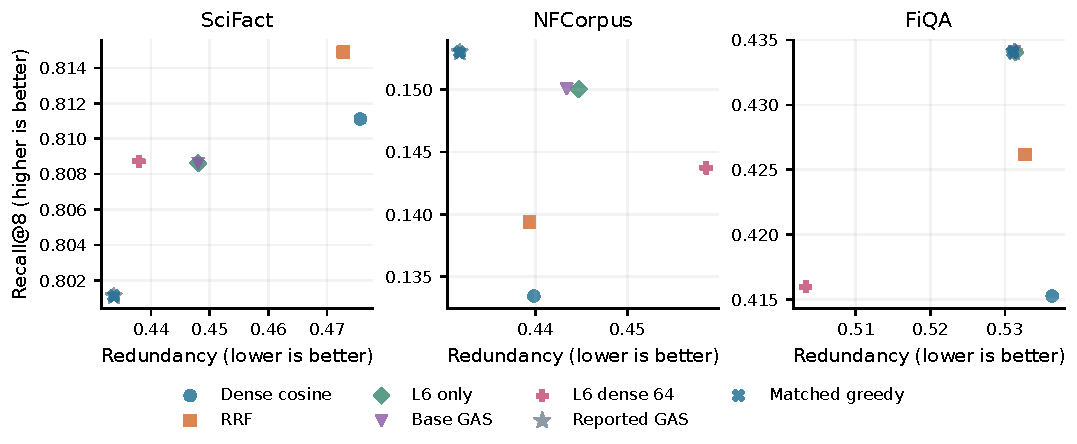
\includegraphics[width=0.98\linewidth]{observed_tradeoffs.pdf}\par
{\fontsize{9.5}{11}\selectfont Figure 1. Recall@8 and redundancy for recorded retrieval policies [10]. Candidate pools differ; coincident points may overlap, and the figure does not establish a universal ranking of methods.\par}\end{center}
Figure 1 shows the relevance-redundancy trade-off: a lower similarity score does not by itself mean that an evidence set contains more judged-relevant material. The protected SciFact and NFCorpus results preserve the first five outputs by construction; the displayed FiQA result uses the earlier base configuration.

The matched greedy and exact-float refiners use the same protected prefix, candidate domain, relevance constraints, and redundancy objective as the refined GAS policy. Their matching aggregate results on SciFact and NFCorpus support the selection formulation; they do not identify an additional effectiveness gain caused by amplitude amplification.

Other comparison points use different candidate pools. A dense-sixty-four cross-encoder sees more initial opportunities than a hybrid-fifteen policy, but it must also score more candidates. The chart is a descriptive view of these recorded configurations, not a controlled comparison that isolates every design choice [10].

\newpage
\reportsubheading{3.5 Query outcomes and resource observations}
Aggregate averages can hide individual losses. Relative to the matched base, protected refinement improved Recall@8 for 2 SciFact queries, left 293 tied, and reduced it for 5. For NFCorpus, 15 queries improved, 295 tied, and 13 declined. Redundancy fell for 158 SciFact and 135 NFCorpus queries and increased for none under the stated acceptance rule [9].

Candidate availability also limits every selector. The average judged Recall@8 ceiling for the hybrid fifteen was 0.8569 on SciFact and 0.1725 on NFCorpus; the expanded union raised those relaxed ceilings to 0.8903 and 0.1942. These are optimistic bounds under the available judgments, not performance guarantees for the constrained policy.

\begin{center}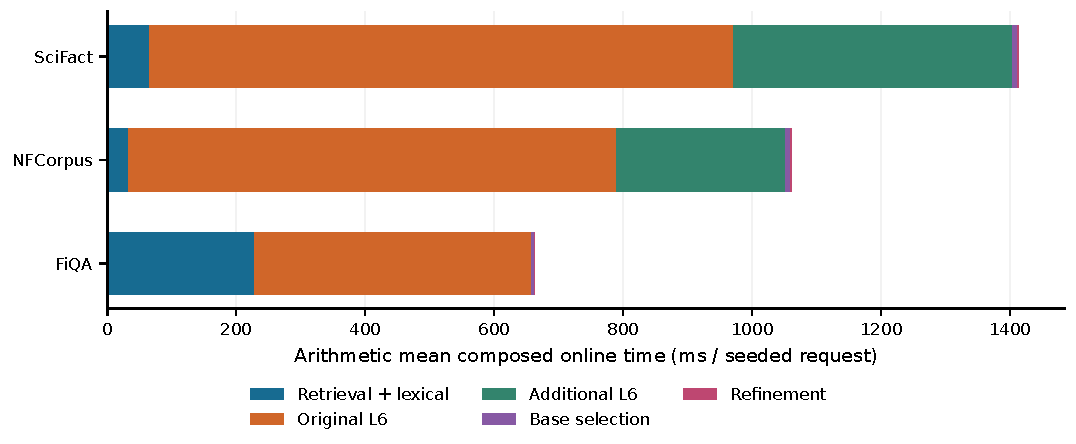
\includegraphics[width=0.98\linewidth]{cost_decomposition.pdf}\par
{\fontsize{9.5}{11}\selectfont Figure 2. Mean composed online time per seeded request, separated into retrieval, neural inference, and selection stages [10]. The FiQA bar represents its earlier base policy.\par}\end{center}
Figure 2 attributes arithmetic mean time to measured stages. Original L6 inference accounts for 64.0\% of the SciFact, 71.3\% of the NFCorpus, and 64.8\% of the FiQA primary means; additional L6 scoring contributes to the two refined pipelines. These are shared-host measurements, not controlled speed comparisons across datasets.

The combined base and refinement selector represents only 0.67\%, 0.88\%, and 0.61\% of those respective mean times. Reducing the selector alone therefore leaves the larger retrieval and neural stages. The compact simulator enumerates its encoded objective and does not demonstrate physical quantum acceleration, energy savings, or a lower monetary cost.

A preserved prefix does not prevent a relevant tail item from being replaced. In one retrospectively selected SciFact case, the only judged-relevant output was lost even though top-five ranking and the candidate-pool ceiling were unchanged. This example illustrates a possible failure mode; it is not representative of every query [10].

The recorded recall-retention gate is a descriptive mean-based criterion, not a prospective statistical noninferiority test. Some confidence intervals include both gains and losses, and the prior use of test outcomes during development limits confirmatory claims. Future studies should retain these negative outcomes and specify success criteria before evaluation.

The hybrid shortlist contained no positively judged parent for 40 SciFact, 91 NFCorpus, and 203 FiQA queries. Selection cannot recover a judged-relevant item that is absent from its input pool; expanding within the dense top 64 can help only when that larger pool already contains the item. These counts depend on the available judgments [10].

\newpage
\reportheading{4. Concluding Remarks}
QubitChat brings document processing, semantic retrieval, cited answer generation, and session management into one prototype. Its research study shows that constrained selection can lower an embedding-based redundancy measure while preserving a chosen ranking prefix. Recall can still decrease, and comparable classical optimizers achieved the same aggregate quality in the protected tests. The results do not establish a physical quantum speedup or an improvement in generated-answer quality.

The evaluation separates guarantees from observations. Protecting the first five positions guarantees the same nDCG@5 as the corresponding base ranking, but score constraints do not guarantee the relevance of a replacement tail. The failed FiQA follow-up and the query-level recall losses demonstrate why both aggregate and individual outcomes matter.

\reportheading{5. Future Work}
Future work should evaluate citation accuracy, answer factuality, and usefulness with real users and diverse uploaded documents. Further retrieval studies should use untouched domains, stronger rerankers, and predefined recall criteria. Improved OCR, multilingual support, and production-scale performance evaluation are also valuable. Any quantum implementation should separately account for state preparation, data access, hardware noise, and end-to-end cost.

A prospective user study could assess whether the cited passages actually support each response and whether readers can locate the evidence efficiently. Retrieval experiments should also compare modern rerankers, measure the full latency of each policy, and report query-level failures rather than relying on a single average.

For the application, further work can examine extraction quality on complex tables, poor scans, and multilingual documents, alongside recovery from processing errors. A production evaluation should measure concurrent use and document lifecycle behavior, and should review the privacy implications of sending retrieved excerpts to an external generation service.

\reportheading{References}
{\raggedright\fontsize{10.3}{11.7}\selectfont [1] P. Lewis et al., "Retrieval-augmented generation for knowledge-intensive NLP tasks," Advances in Neural Information Processing Systems, vol. 33, 2020, pp. 9459-9474.\par}
{\raggedright\fontsize{10.3}{11.7}\selectfont [2] N. Reimers and I. Gurevych, "Sentence-BERT: Sentence embeddings using Siamese BERT-networks," EMNLP-IJCNLP, 2019, pp. 3982-3992. doi:10.18653/v1/D19-1410.\par}
{\raggedright\fontsize{10.3}{11.7}\selectfont [3] S. Robertson and H. Zaragoza, "The probabilistic relevance framework: BM25 and beyond," Foundations and Trends in Information Retrieval, vol. 3, no. 4, 2009, pp. 333-389.\par}
{\raggedright\fontsize{10.3}{11.7}\selectfont [4] R. Nogueira and K. Cho, "Passage re-ranking with BERT," arXiv:1901.04085, 2019.\par}
{\raggedright\fontsize{10.3}{11.7}\selectfont [5] J. Carbonell and J. Goldstein, "The use of MMR, diversity-based reranking for reordering documents and producing summaries," ACM SIGIR, 1998, pp. 335-336.\par}
{\raggedright\fontsize{10.3}{11.7}\selectfont [6] L. K. Grover, "A fast quantum mechanical algorithm for database search," ACM STOC, 1996, pp. 212-219. doi:10.1145/237814.237866.\par}
{\raggedright\fontsize{10.3}{11.7}\selectfont [7] A. Gilliam, S. Woerner, and C. Gonciulea, "Grover Adaptive Search for constrained polynomial binary optimization," Quantum, vol. 5, art. 428, 2021. doi:10.22331/q-2021-04-08-428.\par}
{\raggedright\fontsize{10.3}{11.7}\selectfont [8] N. Thakur et al., "BEIR: A heterogeneous benchmark for zero-shot evaluation of information retrieval models," NeurIPS Datasets and Benchmarks Track, 2021.\par}
{\raggedright\fontsize{10.3}{11.7}\selectfont [9] B. R. Gundapaneni, A. B. Syed, J. Borru, and N. S. Puppala, "Qubit Chat: A Controlled Evaluation of Grover-Inspired Reranking for Document Retrieval," project manuscript and supporting evidence, 2026.\par}
{\raggedright\fontsize{10.3}{11.7}\selectfont [10] B. R. Gundapaneni, A. B. Syed, J. Borru, and N. S. Puppala, "Grover-Inspired Evidence Selection for Document Retrieval: Relevance Constraints, Failure Analysis, and Resource Accounting," journal manuscript and supporting evidence, 2026.\par}
\end{document}
